\documentclass[a4paper,12pt]{article}

\setlength{\oddsidemargin}{0in}
\setlength{\textwidth}{6.5in}    % Decrease the side margins
\usepackage{multirow}
\usepackage{graphicx}

\usepackage{amsmath}

\usepackage[hang, small,labelfont=bf,up,textfont=it,up]{caption} % Custom captions under/above floats in tables or figures
\usepackage{fix-cm}	 % Custom font sizes - used for the initial letter in the document
\setlength{\headheight}{0in}
\setlength{\headsep}{0in}
\setlength{\topmargin}{0in}
\setlength{\textheight}{9in}     % Decrease the top and bottom margins

\title{Parallel Scientific Computing}
\author{Sean Laguna  \\
	\and 
	Hannah Morgan \\
	\and
	Daniel Reid \\
	}
\date{\vspace{-5ex}}	
\begin{document}
%\pagestyle{empty}   % No page numbering
\maketitle



\paragraph*{}
	The purpose of this project is to implement a block inverse method using parallel prefix (PP) to solve a banded lower triangular matrix.  The required time is compared to the time required for solving the matrix using serial forward substitution (FS).  It was found that the total time required to solve a problem once with the block inverse parallel prefix  method was much greater the time to solve using forward substitution.  However much of work done in the PP method is reusable, so the marginal work to solve using the PP method is less than that of FS for large matrices ($n > 512$).
\paragraph*{}
	The algorithm was implemented using two different methods: pthreads and Windows threads.  Both methods use a shared memory model.  The pthread implementation will be tested on the 32-core Computer Science Clover server since they can be compiled for Linux.  The windows thread implementation will be run on an 8-core Windows machine.  The implementations will be timed and compared to the forward substitution method.

\paragraph*{}
	The algorithms were tested on a banded lower triangular matrix of bandwidth 2 as shown in Equation \ref{eq:mtxSetup}.
	\begin{equation} \label{eq:mtxSetup}
		\begin{bmatrix}
		1 & 0 & 0  &  \cdots & 0  \\
		-1  & 1  & 0&   \cdots & 0 \\
		0 & -1 & 1  & \ddots & 0 \\
		\vdots & \vdots & \ddots  & \ddots & \vdots\\
		 0 & 0 & 0 & \cdots &  1  \\
		\end{bmatrix}
		\begin{bmatrix}
		x_1\\
		\vdots \\
		x_i\\
		\vdots \\
		x_n\\
		\end{bmatrix} = 
		\begin{bmatrix}
		1\\
		\vdots \\
		1\\
		\vdots \\
		1\\
		\end{bmatrix}
	\end{equation}
	The equation is abbreviated as $$Lx=f$$
\section*{Windows Thread Implementation}
	\paragraph*{}
		The time to solve the matrix was measured for the parallel prefix and the forward substitution method.  The results are shown in Figure \ref{danielTimes}.  Note that forward substitution was done in serial.  It can be seen that the PP method takes significantly longer than the FS method to solve the matrix once.  However much of the work done on L can be used for multiple X vectors, making the marginal work to solve with the parallel prefix lower than the work for forward substitution for sufficiently large matrices.  Figure \ref{danielMarginal}  compares the marginal time for forward substitution to that of parallel prefix.  
		\begin{figure}[]
			\centering
			\caption{Graph of total time to solve $Lx=f$ using forward substitution and block inverse/parallel prefix and of marginal time to solve block inverse/parallel prefix.  Forward substitution is faster if the problem will only be solved once.}
			\label{danielTimes}
		
			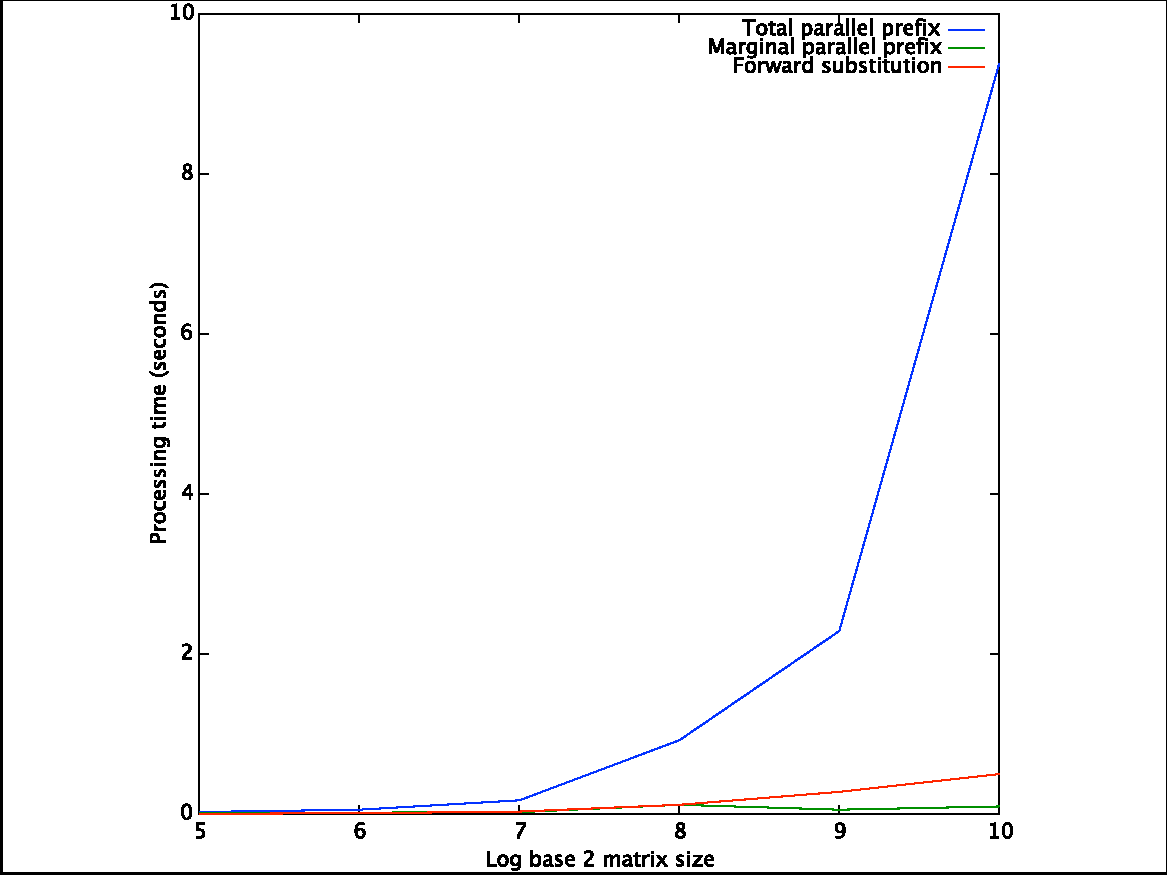
\includegraphics[width=4in]{daniel-times-plot}
		\end{figure}
		\begin{figure}[]
			\centering
			\caption{Graph of marginal time to solve $Lx=f$ using block inverse/parallel prefix and forward substitution.  The marginal time to solve using forward substitution is the same as the total time since no work is reusable.  The BI/PP method is faster for large matrices.}
			\label{danielMarginal}
			
			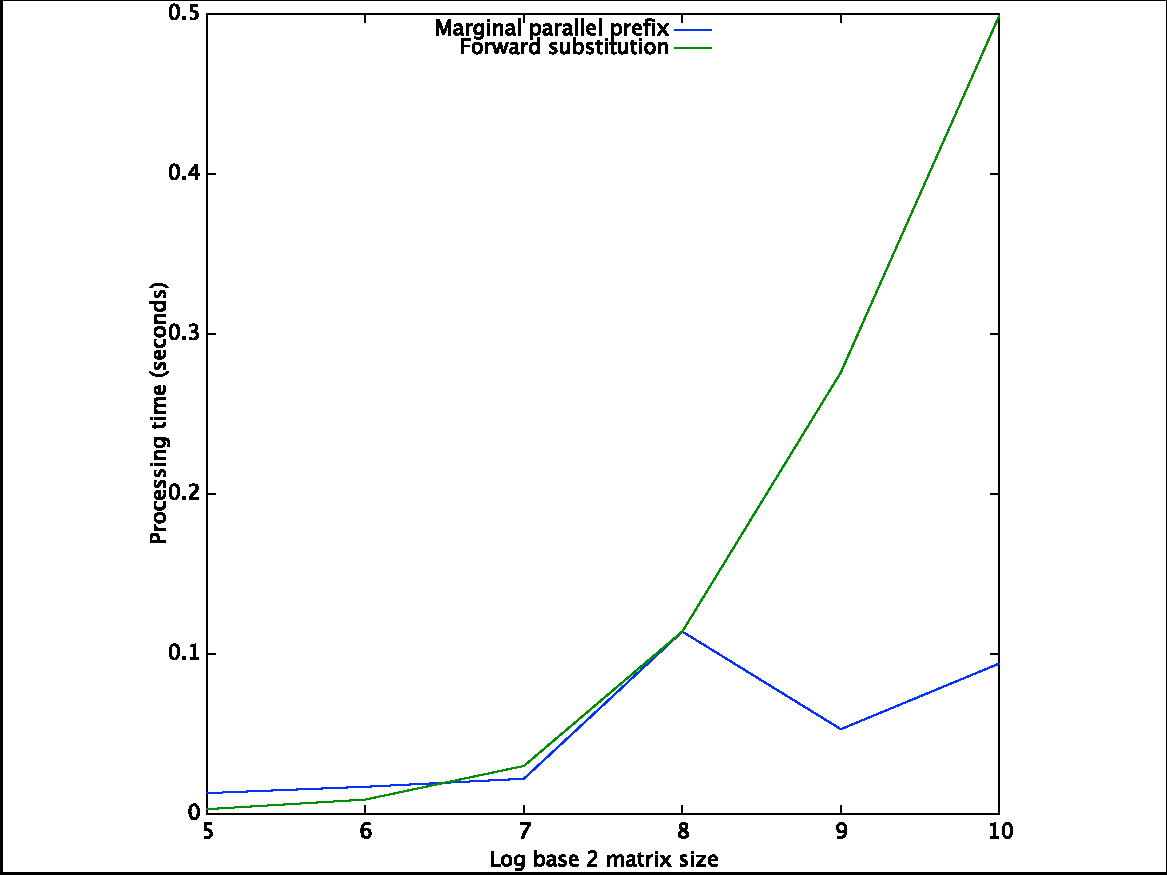
\includegraphics[width=4in]{daniel-plots-marginal}
		\end{figure}
	\paragraph*{}
		Some optimization was done to speed up the process.  The speed increases due to each of the optimizations described are shown in Table SPEEDS Initially, C\verb!++! Vectors were used to store arrays of matrices such as the $Gi$s, $Li$s, etc.  These arrays are all of fixed and known length, so the code was optimized by replacing the vectors with static arrays.  Using static arrays did not noticeably change the runtime for a small number of processors.  This is probably because the C\verb!++! Vector class allocates some number of slots in initialization.  If the final length of the vector is less than that number of slots, the vector will not have to moved in memory.  This could change with more processors.  I used a custom and mostly unoptimized matrix class, which will like give slower runtimes.  
	\paragraph*{}
		Computing the $Gi$s used a large fraction of the total time to set up a problem.  The process was parallelized.  This does not affect the marginal work of solving, but reduces the time to set up and solve a single problem by a factor of 2-3.  Finally, the Matrix class was optimized by reserving array in advance of pushing the values onto it.  This custom matrix class is still slow compared to C\verb!++! libraries such as Eigen, but is suitable for considering relative speeds.   



\end{document}